%%%%%%%%%%%%%%%%%%%%%%%%%%%%%%%%%%%%%%%%%%%%%%%%%%%%%%%%%%%%%%%%%%%%%%%
% BAB 4
%%%%%%%%%%%%%%%%%%%%%%%%%%%%%%%%%%%%%%%%%%%%%%%%%%%%%%%%%%%%%%%%%%%%%%%




% question: perancangan model? atau digabung dengan tahap pelatihan model?


\mychapter{4}{BAB 4 PEMBUATAN MODEL}

Pada bab ini, dijelaskan tahapan pembuatan model yang digunakan dalam penelitian ini. Tahapan pembuatan model meliputi \textit{preprocessing} data, ekstraksi fitur, pelatihan model, dan evaluasi model. Gambar \ref{fig:alur-model} menunjukkan alur pembuatan model yang digunakan dalam penelitian ini.

\begin{figure}[H]
  \begin{center}
    \includegraphics[width=1\textwidth]{img/lstm-ML Pipeline.drawio.pdf}
  \end{center}
  \caption{Alur pembuatan model}
  \label{fig:alur-model}
\end{figure}

\section{\emph{Preprocessing} Data}
\label{subsec: bab4-preprocessing-data}

Dataset yang digunakan dalam penelitian ini diperoleh dari MIT-BIH Arrhythmia Database.
Sebelum data dapat digunakan untuk pelatihan model, data ECG harus melalui tahap \textit{preprocessing}.
\textit{Preprocessing} dilakukan untuk memastikan kualitas dan keandalan data yang digunakan dalam proses pelatihan model. 
Terdapat beberapa tahap \textit{preprocessing} yang dilakukan pada penelitian ini, yaitu pemetaan dataset, penghapusan \textit{noise} berfrekuensi tinggi, penghapusan \textit{baseline wander} (BW), dan normalisasi.

Data ECG pada MIT-BIH Arrhythmia Database memiliki anotasi yang terdiri dari 20 kelas, sedangkan pada penelitian ini hanya menggunakan 5 kelas yaitu Normal (N), \textit{Supraventricular Ectopic Beat} (S), \textit{Ventricular Ectopic Beat} (V), \textit{Fusion} (F), dan \textit{Unknown} (Q).
Kelas-kelas tersebut dipilih berdasarkan rekomendasi dari Association for the Advancement of Medical Instrumentation (AAMI), yang mengelompokkan berbagai jenis aritmia ke dalam kategori yang lebih umum.
Oleh karena itu, perlu dilakukan pemetaan kelas pada dataset agar sesuai dengan kelas yang digunakan pada penelitian ini.
Pemetaan tersebut dapat dilihat pada Tabel \ref{tab:aami-label}, yang menunjukkan bagaimana kelas-kelas dari dataset dipetakan ke dalam 5 kelas yang digunakan dalam penelitian ini.

\begin{table}[h]
	\caption{Kelas Rekomendasi AAMI dan Simbol pada MIT-BIH}
	\begin{center}
		\begin{tabular}{c @{\hspace{1cm}} c}
			\hline
			AAMI                              & MIT-BIH       \\
			\hline
			Normal (N)                        & N, L, R, e, j \\
                        \textit{Supraventricular Ectopic Beat} (S) & A, a, J, S    \\
                        \textit{Ventricular Ectopic Beat} (V)      & V, E          \\
                        \textit{Fusion} (F)                        & F             \\
                        \textit{Unknown} (Q)                       & /, f, Q       \\
			\hline
		\end{tabular}
	\end{center}
	\label{tab:aami-label}
\end{table}

% metode penghilangan frekuensi tinggi
%     ecg = denoise_wavelet(ecg, method='VisuShrink', mode='soft', wavelet_levels=10, wavelet='db8', rescale_sigma='True')

% Selama proses pengambilan data, sinyal ECG dapat terganggu oleh \textit{noise} berfrekuensi tinggi.
Selama proses pengambilan data, sinyal ECG rentan terhadap \textit{noise} berfrekuensi tinggi.
% Frekuensi tinggi pada data ECG dianggap sebagai \textit{noise} yang dapat mengganggu proses klasifikasi detak jantung.
% Oleh karena itu, perlu dilakukan penghilangan \textit{noise} berfrekuensi tinggi pada data ECG.
Frekuensi tinggi pada data ECG dianggap sebagai \textit{noise} yang dapat mengganggu proses klasifikasi detak jantung, sehingga perlu dilakukan penghilangan \textit{noise} tersebut.
Pada penelitian ini, \textit{noise} berfrekuensi tinggi dihilangkan dengan menggunakan metode \textit{wavelet denoise}.
\textit{Wavelet denoise} merupakan metode yang digunakan untuk menghilangkan \textit{noise} pada sinyal maupun gambar dengan menggunakan \textit{wavelet transform}.
\textit{Wavelet transform} memungkinkan sinyal untuk dipecah menjadi beberapa bagian frekuensi yang berbeda, sehingga memungkinkan penghilangan \textit{noise} pada frekuensi tertentu.
Metode \textit{wavelet denoise} yang digunakan pada penelitian ini adalah \textit{VisuShrink} dengan mode \textit{soft thresholding}, dan menggunakan \textit{wavelet} Daubechies 8 (db8) dengan 10 level \textit{wavelet decomposition}.

% --- dijelaskan lebih detail? ---

% Sinyal ECG diubah ke dalam domain \textit{wavelet} dengan menggunakan \textit{wavelet transform} Daubechies 8 (db8) dengan 10 level \textit{wavelet decomposition}.
% \textit{Noise} pada sinyal ECG kemudian dapat dihilangkan dengan mengurangi koefisien \textit{wavelet} yang memiliki nilai di bawah ambang batas tertentu.

%
% Setelah menghilangkan \textit{noise} berfrekuensi tinggi, tahap selanjutnya adalah menghilangkan \textit{baseline wander} (BW).
% elaborate
Selain \textit{noise} berfrekuensi tinggi, sinyal ECG juga rentan terhadap
baseline wander.
\textit{Baseline wander} (BW) merupakan \textit{noise} berfrekuensi rendah yang terdapat pada ECG.
BW dapat disebabkan oleh beberapa faktor, seperti pernapasan, elektroda yang bermuatan listrik, dan gerakan dari pasien \parencite{lenisComparisonBaselineWander2017}.
% metode baseline wander
        % baseline = medfilt(ecg, 71)
        % baseline = medfilt(baseline, 215)
        %
        % # Remove Baseline
        % for i in range(0, len(ecg)):
        %     ecg[i] = ecg[i] - baseline[i]
% BW dihilangkan dengan menggunakan metode \textit{median filter} dengan panjang jendela 71 dan 215.
BW dihilangkan dengan melakukan substraksi antara sinyal ECG dengan \textit{trend} sinyal.
\textit{Trend} sinyal diperoleh dengan menggunakan metode \textit{median filter} sebanyak dua kali dengan panjang jendela 71 dan 215.
% Median filtering, as mentioned earlier, is another method commonly used for baseline wander removal. It involves replacing each data point in the signal with the median value within a specified window around that point. This approach can effectively remove baseline variations while preserving the shape of the ECG waveform.
\textit{Median filter} akan menggantikan setiap titik data pada sinyal dengan nilai median dalam jendela yang ditentukan.
\textit{Median filter} didefinisikan oleh persamaan \ref{eq:median-filter}.
\begin{equation}
    % perlu dicek lagi
    y[n] = \text{median}(x[n - \frac{M}{2} : n + \frac{M}{2}])
    \label{eq:median-filter}
\end{equation}
Yang mana $y[n]$ adalah sinyal hasil \textit{median filter}, $x[n]$ adalah sinyal asli, dan $M$ adalah panjang jendela \textit{median filter}.

% Setelah \textit{baseline wander} dihilangkan, data dinormalisasi untuk menghindari perbedaan skala.
% Setelah \textit{nose} dan \textit{baseline wander} dihilangkan, data dinormalisasi untuk menghindari perbedaan skala.
% Normalisasi yang dilakukan yaitu \textit{Z-score normalization}.
% metode normalisasi
Setelah \textit{noise} dan \textit{baseline wander} dihilangkan, tahap selanjutnya adalah normalisasi data.
Normalisasi dilakukan untuk menghindari adanya perbedaan skala pada data.
Metode normalisasi yang digunakan pada penelitian ini adalah \textit{Z-score normalization}.
\textit{Z-score normalization} mengubah data ke dalam distribusi normal dengan rata-rata 0 dan standar deviasi 1.
\textit{Z-score normalization} didefinisikan oleh persamaan \ref{eq:z-score}.
\begin{equation}
		z = \frac{x - \mu}{\sigma}
		\label{eq:z-score}
\end{equation}
Yang mana $z$ adalah data yang telah dinormalisasi, $x$ adalah data asli, $\mu$ adalah rata-rata data, dan $\sigma$ adalah standar deviasi data.


% Gambar \ref{fig:sebelum-prep} menunjukkan data sebelum dilakukan \textit{preprocessing}, sedangkan Gambar \ref{fig:setelah-prep} menunjukkan data setelah dilakukan \textit{preprocressing}.
Gambar \ref{fig:sebelum-prep} dan \ref{fig:setelah-prep} memperlihatkan perbandingan data ECG sebelum dan setelah dilakukan \textit{preprocessing}.
% Pada Gambar \ref{fig:sebelum-prep}, terlihat bahwa terdapat \textit{noise} berfrekuensi tinggi dan variasi pada \textit{baseline} sinyal ECG.
Pada Gambar \ref{fig:sebelum-prep}, terlihat bahwa data ECG masih mengandung gangguan seperti \textit{noise} berfrekuensi tinggi dan variasi pada \textit{baseline} sinyal.
% Setelah dilakukan \textit{preprocessing}, sinyal ECG menjadi lebih halus dan memiliki baseline yang lebih rata.
Setelah dilakukan \textit{preprocessing}, sinyal ECG menjadi lebih halus dan memiliki \textit{baseline} yang lebih rata, seperti yang terlihat pada Gambar \ref{fig:setelah-prep}.

\begin{figure}[H]
    \centering
    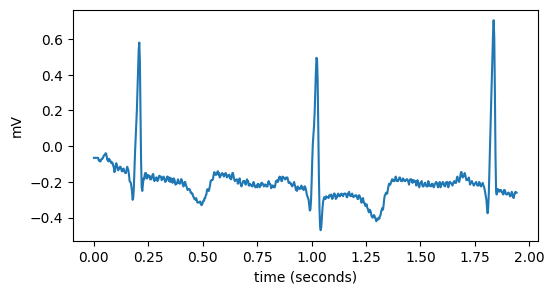
\includegraphics[width=0.6\linewidth]{./img/sebelum_prep.png}
	\caption{Data sebelum \textit{preprocessing}}
	\label{fig:sebelum-prep}
\end{figure}

\begin{figure}[H]
  \centering
  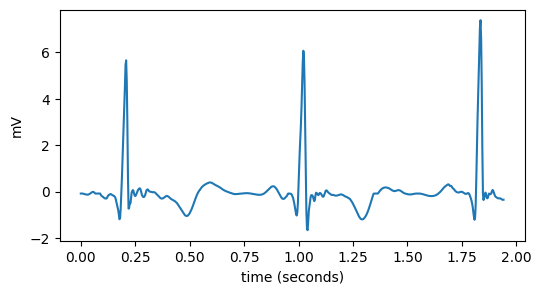
\includegraphics[width=0.6\linewidth]{./img/setelah_prep.png}
  \caption{Data setelah \textit{preprocessing}}
  \label{fig:setelah-prep}
\end{figure}


\section{Ekstraksi Fitur}
\label{subsec: bab4-ekstraksi-fitur}

Kami menggunakan RR-Interval sebagai fitur dalam penelitian ini.
% taruh sini atau bab 2?
RR-Interval adalah jarak antara dua titik R pada sinyal ECG.
Visualisasi dari RR-Interval ditunjukkan oleh Gambar \ref{fig:rri}.
Dari interval RR ini, kami mengekstraksi 9 fitur, yaitu RR0, RR-1, RR+1, RR0/avgRR, tRR0, RR-1/avgRR, RR-1/RR0, RR+1/avgRR, dan RR+1/RR0 \parencite{pramukantoroHeartbeatClassifierContinuous2022}.
Tabel \ref{tab:rri} menunjukkan deskripsi lengkap dari setiap fitur.
Ekstraksi dilakukan dengan jendela sepanjang 42 data. Rata-rata RR-Interval (avgRR) merupakan rata-rata dari 42 data, termasuk RR-0. 

\begin{figure}[H]
  \centering
  \includegraphics[scale=.7]{img/lstm-Page-7.drawio.pdf}
  \caption{RR-Interval}
  \label{fig:rri}
\end{figure}

\begin{table}[H]
  \caption{Deskripsi RR-Interval}
\begin{center}
\footnotesize
\begin{tabular}{c @{\hspace{1cm}} c}
\hline
Fitur & Deskripsi\\
\hline
RR0 & Nilai RRi saat ini\\
RR-1 & Nilai RRi sebelumnya\\
RR+1  & Nilai RRi selanjutnya\\
RR0/avgRR & Nilai RRi saat ini dibagi dengan rata-rata 42 RRi sebelumnya\\
tRR0  & (RRi saat ini - rata-rata RRi) / stddevRRi\\
RR-1/avgRR & Nilai RRi sebelumnya / rata-rata RRi\\
RR-1/RR0 & Nilai RRi sebelumnya / RRi saat ini\\
RR+1/avgRR & Nilai RRi selanjutnya / rata-rata RRi\\
RR+1/RR0 & Nilai RRi selanjutnya / RRi saat ini\\
\hline
\end{tabular}
\end{center}
\center
Sumber: \textcite{pramukantoroHeartbeatClassifierContinuous2022}
\label{tab:rri}
\end{table}

%contoh extracted feature

% considering cuma pakai lstm256 tapi dengan fitur lain
\section{Perancangan Model LSTM}
\label{subsec: bab4-pembuatan-model-lstm}
Pada tahap ini, penulis membuat model berbasis LSTM yang akan digunakan untuk melakukan klasifikasi detak jantung. 
% Dalam penelitian ini, 
Terdapat tiga jenis model yang akan digunakan pada penelitian, yaitu \textit{Long Short-Term Memory} (LSTM), \textit{Bidirectional} LSTM (Bi-LSTM), serta LSTM \textit{Fully Convolutional Network} (LSTM-FCN). 
Pembuatan model meliputi pembuatan arsitektur model, pelatihan model, dan evaluasi model.
Model dibuat dengan menggunakan \textit{framework} TensorFlow dan dilatih sebanyak 50 \textit{epoch}.


% LSTM merupakan pengembangan dari \textit{Recurrent Neural Network} (RNN) yang dirancang untuk mengatasi masalah yang umum terjadi pada RNN tradisional, yaitu hilangnya informasi masa lalu \parencite{hochreiterLongShorttermMemory1997}.  LSTM memiliki kemampuan untuk mengingat informasi yang disimpan dalam jangka waktu yang lama. 


Arsitektur model LSTM yang digunakan dalam penelitian ini ditunjukkan oleh Gambar \ref{fig:arslstm}. Model terdiri dari tiga \textit{layer}, yakni satu buah LSTM \textit{layer} dan dua buah \textit{dense layer}. Terdapat dua varian model LSTM yang dilatih dengan menggunakan dua \textit{hyperparameter} berbeda. Model pertama memiliki 512 unit LSTM pada \textit{layer} pertama dan 256 unit \textit{dense} pada \textit{layer} kedua. Sementara itu, model kedua memiliki 256 unit LSTM pada layer pertama dan 128 unit \textit{dense} pada \textit{layer} kedua.

% img arsi lstm
\begin{figure}[H]
  \centering
  \includegraphics[scale=1, angle=-90]{img/lstm-Page-2.drawio.pdf}
  \caption{Arsitektur LSTM}
  \label{fig:arslstm}
\end{figure}

\textit{Bidirectional} LSTM atau Bi-LSTM merupakan pengembangan dari LSTM yang dapat dilatih dua arah secara bersamaan dengan \textit{hidden layer} yang terpisah \parencite{yuReviewRecurrentNeural2019}. Dengan menggabungkan LSTM dengan \textit{bidirectional} RNN, Bi-LSTM mampu mengatasi keterbatasan LSTM konvensional yang hanya dapat memanfaatkan informasi sebelumnya. Gambar \ref{fig:arsbilstm} menunjukkan arsitektur model Bi-LSTM yang digunakan dalam penelitian ini.

% img arsi bi-lstm
\begin{figure}[H]
  \centering
  \includegraphics[scale=1, angle=-90]{img/lstm-Page-3.drawio.pdf}
  \caption{Arsitektur Bi-LSTM}
  \label{fig:arsbilstm}
\end{figure}

LSTM-FCN atau LSTM-\textit{Fully Convolutional Network} merupakan model gabungan antara LSTM dengan  \textit{Fully Convolutional Network} (FCN) \parencite{karimLSTMFullyConvolutional2018}. Arsitektur model ini terdiri dari dua blok, yaitu blok \textit{convolutional} dan blok LSTM. Blok \textit{convolutional} terdiri dari tiga \textit{layer convolutional} 1 dimensi, sedangkan blok LSTM hanya terdiri dari satu layer LSTM. Pada versi original, untuk menghindari \textit{overfitting}, terdapat \textit{dimension shuffle} yang akan mengacak input sebelum blok LSTM. Akan tetapi, meletakkan \textit{dimension shuffle} sebelum blok LSTM akan menyebabkan hilangnya informasi pada dimensi waktu \parencite{8713870}. Pada penelitian ini kami melakukan modifikasi pada LSTM-FCN dengan menukar posisi \textit{dimension shuffle} pada sebelum blok \textit{convolutional}. Gambar \ref{fig:arslstmfcn} menunjukkan struktur model LSTM-FCN modifikasi yang digunakan pada penelitian.

% img arsi lstm-fcn
\begin{figure}[H]
  \centering
  \includegraphics[scale=0.7, angle=-90]{img/lstm-Page-4.drawio.pdf}
  \caption{Arsitektur LSTM-FCN Modifikasi}
  \label{fig:arslstmfcn}
\end{figure}

\section{Pelatihan Model}

Seluruh model dilatih dengan menggunakan \textit{framework} TensorFlow. 
Pelatihan dilakukan dengan menggunakan dataset yang telah dilakukan \textit{preprocessing} dan ekstraksi fitur sebelumnya.
Pelatihan dilakukan sejumlah 50 \textit{epoch} dengan menggunakan ukuran \textit{batch} 256.
Selama proses pelatihan, digunakan algoritma optimasi Adam dengan \textit{learning rate} 0.001.
Model dilatih pada perangkat server DGX A100.

\section{Evalusi Model}

\begin{table}[ht]
\caption{Evaluasi Model}
\label{hasilLSTM}
\begin{center}
\begin{tabular}{cccccc}
\hline
\multicolumn{1}{c}{Fitur} 
 & \multicolumn{1}{c}{Model}
 & \\
\hline
 & & Akurasi & \emph{Precision} & \emph{Recall} & F1-\emph{score} \\
\hline
\multirow{3}{4em}{RRI} & LSTM 512 & 0.9679 & 0.9662  & 0.9679 &  0.9652 \tabularnewline
& LSTM 256 & 0.9674 & 0.9656 &  0.9674 &  0.9645 \tabularnewline
& Bi-LSTM & 0.9636 & 0.9617  & 0.9636 &  0.9606 \tabularnewline
& LSTM-FCN & 0.9667 & 0.9643 &  0.9667  & 0.9643 \tabularnewline
\hline
\end{tabular}
\end{center}
\end{table}
